% ================================================================= C3: KẾT QUẢ PROTOTYPE
\section{Đóng góp C3 sau khi chạy prototype}
\label{sec:fsqi}

Bản đề cương trước đặt C3 là ``chỉ số chất lượng tín hiệu thai dựa trên đồng điều bền vững, có quyền
từ chối trả lời'' và thừa nhận nó chưa có một dòng dữ liệu nào. Nhóm đã xây prototype và chạy thí nghiệm
có kiểm soát. \textbf{Kết quả là phủ định cho phần đồng điều bền vững, và khẳng định cho phần từ chối
trả lời.} Mục này trình bày nguyên trạng.

\subsection{Thiết kế thí nghiệm}

Câu hỏi: \textit{đặc trưng topo tính trên từng đoạn 4 giây có dự báo được khi nào mô hình sẽ sai không,
và có hơn các chỉ số chất lượng cổ điển không?}

\begin{table}[H]\centering\small
\caption{Hai nhóm đặc trưng được so sánh. Mọi đặc trưng tính trên tín hiệu dư sau khử mẹ, 250\,Hz, đoạn
4 giây, chuẩn hoá robust. Mã tại \texttt{fsqi/fsqi.py}.}
\label{tab:fsqi_dactrung}
\begin{tabular}{@{}L{3.4cm} C{1.0cm} L{9.8cm}@{}}
\toprule
\textbf{Nhóm} & \textbf{Số} & \textbf{Nội dung} \\
\midrule
Topo --- Takens + ripser & 11 & Nhúng trễ chiều 3, $\tau = 20$\,ms, 300 điểm; tổng, cực đại, entropy và
số thanh persistence của $H_0$ và $H_1$ \\
Topo --- sublevel $H_0$ & 5 & Đồng điều $H_0$ của lọc dưới mức trên tín hiệu 1 chiều (đối chiếu với
\texttt{scipy} prominence: sai lệch 0,0 trên 2.011 đỉnh) \\
Cổ điển --- chỉ tín hiệu & 6 & SampEn, kurtosis, entropy phổ, tỉ lệ năng lượng 10--60\,Hz, đỉnh PSD dải
nhịp thai, trễ tự tương quan \\
Cổ điển --- đầu ra mô hình & 6 & CV khoảng RR, tỉ lệ RR hợp lý, bSQI, số đỉnh, xác suất trung bình tại
đỉnh, xác suất cực đại \\
\bottomrule
\end{tabular}
\end{table}

Giao thức chống rò rỉ: nhãn ``đoạn lỗi'' là F1 của mô hình trên đoạn đó dưới 80; bộ phân loại huấn luyện
\textbf{chỉ trên ADFECGDB} (1.500 đoạn, checkpoint fold đúng), kiểm thử \textbf{xuyên miền trên CinC 2013}
(600 đoạn, checkpoint production, zero-shot). Không chọn siêu tham số bằng nhãn kiểm thử. Bootstrap 1.000
lần theo đoạn và theo cụm bản ghi. Hai lần chạy độc lập cho kết quả trùng khớp 1.327/1.327 trường.

\subsection{Kết quả}

\begin{table}[H]\centering\small
\caption{Dự báo đoạn lỗi trên CinC 2013 (ngoài miền), bộ phân loại huấn luyện trên ADFECGDB. Cột cuối:
macro F1 của các đoạn được giữ lại sau khi từ chối 20\% đoạn kém tin cậy nhất.}
\label{tab:fsqi_kq}
\begin{tabular}{@{}L{4.6cm} C{1.9cm} C{1.9cm} C{2.3cm} C{2.3cm}@{}}
\toprule
\textbf{Nhóm đặc trưng} & \textbf{AUROC} & \textbf{AUPRC} & \textbf{F1, phủ 80\%} & \textbf{F1, phủ 50\%} \\
\midrule
Từ chối ngẫu nhiên (đường cơ sở) & 0,500 & $\approx$0,52 & 62,03 & 62,14 \\
\textbf{Topo} (16 đặc trưng) & \xau{0,566} & 0,564 & 63,40 & 64,44 \\
Cổ điển, chỉ tín hiệu (6) & 0,666 & 0,686 & --- & --- \\
\textbf{Cổ điển} (12) & \tot{0,929} & 0,927 & \tot{69,40} & \tot{84,51} \\
Kết hợp topo + cổ điển (28) & 0,905 & 0,899 & 69,41 & 82,44 \\
Oracle (biết F1 thật) & --- & --- & 74,55 & 97,81 \\
\bottomrule
\end{tabular}
\end{table}

\begin{figure}[H]\centering
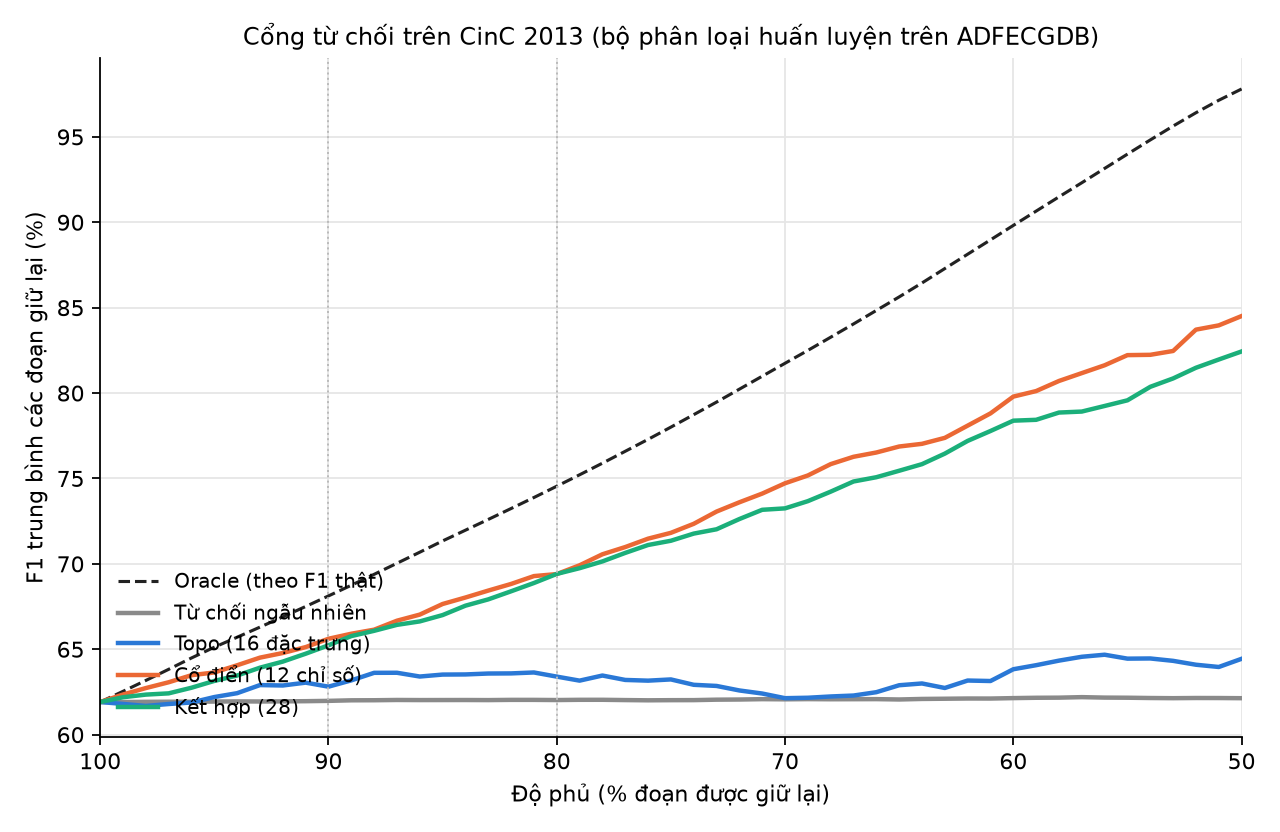
\includegraphics[width=0.92\textwidth]{figs/fig9_risk_coverage.png}
\caption{Đường cong rủi ro--độ phủ trên CinC 2013. Đường topo (xanh dương) gần như nằm sát đường từ chối
ngẫu nhiên (xám) trên toàn bộ dải độ phủ. Đường cổ điển (cam) tách rõ và tiến về oracle (đứt).}
\label{fig:riskcov}
\end{figure}

\begin{figure}[H]\centering
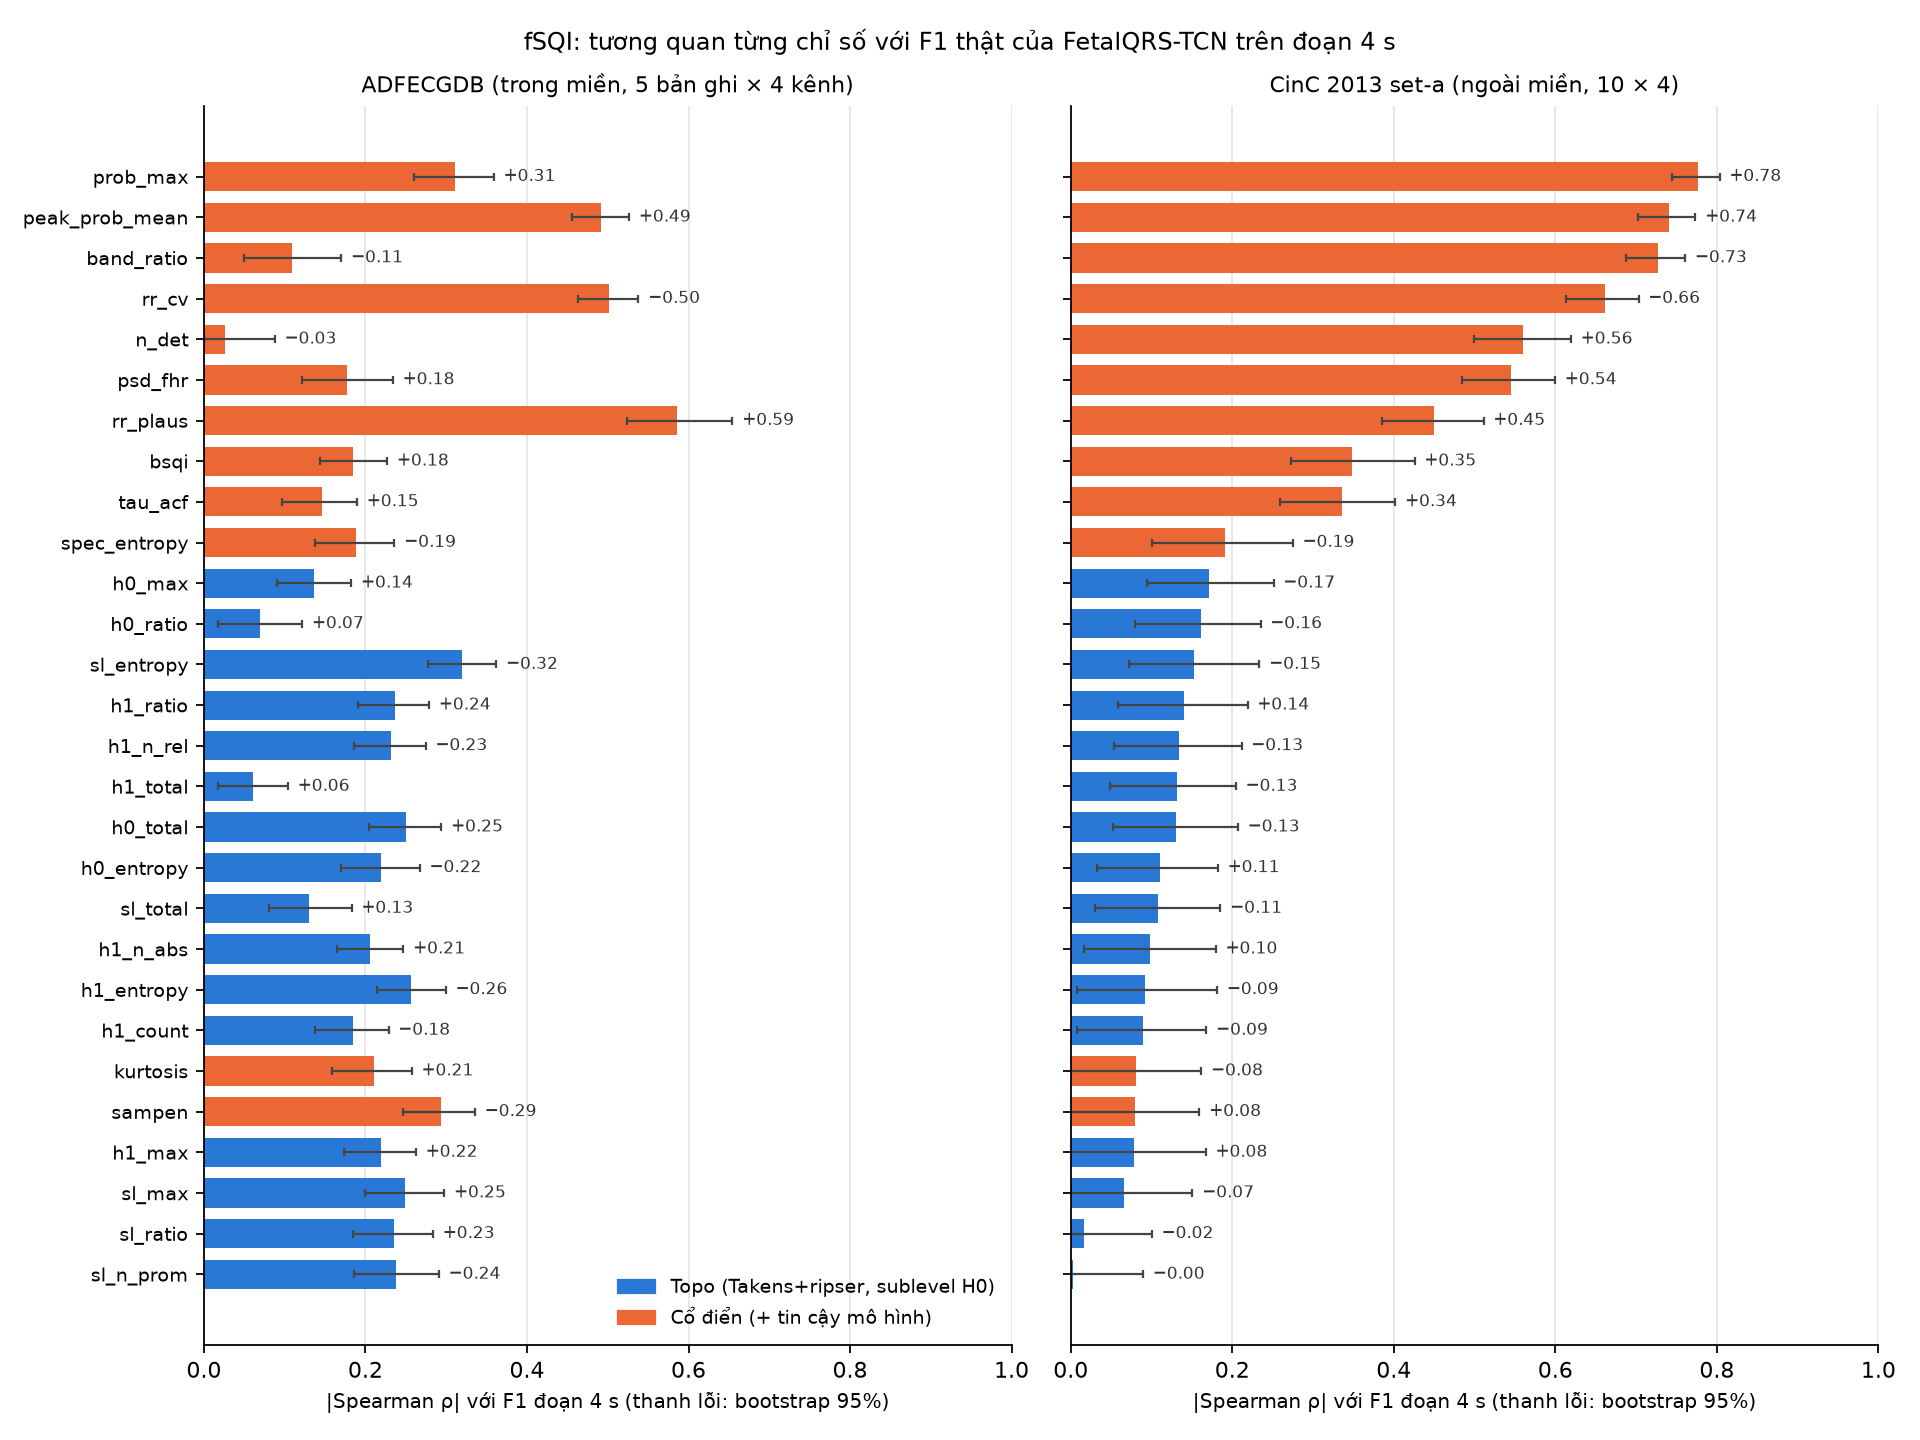
\includegraphics[width=\textwidth]{figs/fig10_sqi_correlation.png}
\caption{Tương quan Spearman của từng chỉ số với F1 đoạn, kèm khoảng tin cậy bootstrap 95\%. Trái: trong
miền. Phải: ngoài miền. Các chỉ số cổ điển (cam) \textbf{mạnh lên} khi ra ngoài miền; các chỉ số topo
(xanh) \textbf{yếu đi} và nhiều chỉ số đổi dấu.}
\label{fig:sqicorr}
\end{figure}

\subsection{Đọc kết quả}

\begin{enumerate}[leftmargin=1.6em,itemsep=5pt]
\item \textbf{Topo không dự báo được lỗi ở mức hữu dụng.} AUROC 0,566 gần ngẫu nhiên. Cổng từ chối dựa
trên topo chỉ hơn từ chối ngẫu nhiên 1,4 điểm ở độ phủ 80\%. Trong miền có tín hiệu yếu ($\rho = -0{,}32$
cho entropy sublevel), nhưng tín hiệu đó \textbf{không chuyển miền được}: bốn đặc trưng topo đổi dấu
tương quan giữa ADFECGDB và CinC.

\item \textbf{Topo không bổ sung gì cho cổ điển.} Gộp 28 đặc trưng cho AUROC 0,905, \textit{thấp hơn} 12
đặc trưng cổ điển đơn thuần (0,929). Thêm topo vào là thêm nhiễu.

\item \textbf{Ngay cả chỉ số cổ điển thuần tín hiệu cũng hơn topo} (0,666 so với 0,566), dù không dùng
đầu ra mô hình.

\item \textbf{Cổng từ chối có tác dụng thật, nhưng bằng chỉ số khác.} Chỉ số dự báo lỗi mạnh nhất là
\textbf{độ tự tin của chính mô hình} (\texttt{prob\_max}, AUROC đơn lẻ 0,970) và \textbf{độ đều của nhịp}
(\texttt{rr\_cv}, 0,915). Chỉ số thuần tín hiệu tốt nhất là \textbf{tỉ lệ năng lượng 10--60\,Hz}
(0,904) --- lần thứ ba dải tần này xuất hiện như biến quan trọng nhất của đề tài.

\item \textbf{Chi phí tính topo không phải rào cản.} Trung bình 65\,ms mỗi đoạn, p95 80\,ms. Vấn đề không
phải tốc độ mà là thông tin.
\end{enumerate}

\begin{canhbao}[title={Con số 0,929 trả lời sai câu hỏi --- đính chính bắt buộc của bản 3.3}]
600 đoạn 4 giây trong bảng trên đến từ \textbf{10 bản ghi}, và đoạn trong cùng một bản ghi tương quan
mạnh. Tính lại với cluster bootstrap \textbf{theo bản ghi} ($n = 10$ cụm): AUROC $= 0{,}929$
$[0{,}830;\ 0{,}982]$.

Quan trọng hơn: \textbf{5/10 bản ghi CinC không có đoạn xấu nào}, nên chúng không đóng góp gì vào AUROC
gộp. Con số 0,929 vì vậy phần lớn trả lời câu hỏi \textit{``bản ghi này có phải bản ghi xấu không''}.
Câu hỏi mà cổng từ chối được bán như là thứ trả lời --- \textit{``đoạn 4 giây này trong bản ghi của bệnh
nhân này có đáng tin không''} --- có đáp số là \textbf{AUROC TRONG bản ghi $= 0{,}721$}
$[0{,}517;\ 0{,}898]$, trung bình trên 5 bản ghi có cả đoạn tốt lẫn đoạn xấu (a01 $= 0{,}914$;
a06 $= 0{,}390$; a07 $= 0{,}889$; a09 $= 0{,}886$; a10 $= 0{,}526$).

Kết luận phủ định về topo \textbf{không đổi} (0,566 so với 0,929 hay so với 0,721 đều là thua). Nhưng
tuyên bố khẳng định về cổng từ chối phải hạ xuống: nó \textbf{chưa} dùng được ở mức đoạn tại giường bệnh.
Chi tiết ở \S\ref{sec:thongke}.
\end{canhbao}

\begin{canhbao}[title={Điều này làm gì với đóng góp C3}]
Nhóm \textbf{rút lại} phần ``dựa trên đồng điều bền vững'' trong phát biểu C3. Đây là lần thứ ba trong đề
tài mà phân tích dữ liệu topo được kiểm chứng có kiểm soát và không mang lại lợi ích: (1) Persistence
Image làm đặc trưng dò đỉnh đứng chót 16 kiến trúc; (2) sublevel $H_0$ trùng 100\% với độ nhô đỉnh cổ
điển; (3) đặc trưng topo làm chỉ số chất lượng đạt AUROC 0,566 so với 0,929 của chỉ số cổ điển.

\textbf{C3 được phát biểu lại thành:} \textit{cổng từ chối trả lời cho bộ dò fQRS đơn kênh, xây trên độ
tự tin của mô hình và tính hợp lý của nhịp, kèm một kết quả phủ định có kiểm soát về đồng điều bền vững
trong vai trò chỉ số chất lượng tín hiệu thai.}

Giả thuyết H0 trong bản đề cương trước đã dự phòng đúng tình huống này: kết quả phủ định có kiểm định,
với đối chứng ngẫu nhiên và oracle, huấn luyện--kiểm thử xuyên miền, không chọn siêu tham số bằng nhãn
kiểm thử, là một đóng góp công bố được.
\end{canhbao}

\subsection{Vì sao topo thất bại ở đây}

Nhóm đưa ra ba lý do, đánh dấu rõ mức chắc chắn:

\begin{description}[leftmargin=2.0em,style=nextline,itemsep=4pt]
\item[Đã chứng minh --- sublevel $H_0$ không phải đặc trưng mới.] Định lý Elder cho biết persistence của
mỗi thanh $H_0$ đúng bằng độ nhô của một đỉnh. Nhóm đã kiểm chứng sai lệch 0,0 trên 2.011 đỉnh. Nên
nhóm 5 đặc trưng này chỉ là cách viết lại thống kê độ nhô, và độ nhô đã nằm trong bộ chỉ số cổ điển.

\item[Đã đo --- đặc trưng $H_1$ của nhúng trễ không ổn định giữa bộ dữ liệu.] Hình \ref{fig:sqicorr} cho
thấy dấu tương quan đổi chiều. Cấu trúc vòng trong không gian nhúng phụ dấu vào biên độ tương đối của
sóng mẹ còn sót và nhiễu cơ, hai thứ khác hẳn giữa hai bộ dữ liệu.

\item[Suy luận --- lỗi mô hình là lỗi \textit{nhịp}, không phải lỗi \textit{hình dạng}.] Ảnh chụp demo
trên a02 (hình \ref{fig:demo_a02}) cho thấy cơ chế thất bại chính: mô hình bám nhầm vào nhịp mẹ. Đó là
lỗi ở thang thời gian hàng giây, trong khi đặc trưng topo trên đoạn 4 giây mô tả hình dạng ở thang mili
giây. Hai thang không gặp nhau. Đây là lý do độ đều nhịp và tỉ lệ trùng đỉnh mẹ dự báo lỗi tốt hơn nhiều.
\end{description}

\subsection{Giới hạn của thí nghiệm này}

CinC 2013 set-a chỉ có 10 bản ghi $\times$ 1 phút, lỗi tập trung theo bản ghi nên khoảng tin cậy theo cụm
rộng hơn nhiều so với theo đoạn. Chỉ một cấu hình topo được thử (chiều 3, $\tau = 20$\,ms, 300 điểm) và
nhóm \textbf{cố ý không quét} tham số để tránh chọn theo nhãn kiểm thử --- nên chưa loại trừ hoàn toàn
khả năng một cấu hình khác tốt hơn. Bộ phân loại kết hợp (0,905) thấp hơn cả \texttt{prob\_max} đơn lẻ
(0,970), tức một ngưỡng đơn có thể là cổng tốt hơn bộ học, và điều này chưa được đo riêng.
